%%%%%%%%%%%%%%%%%%%%%%%%%%%%%%%%%%%%%%%%%%%%%%%%%%%%%%%%%%%%%%%%%%%%%%%%%%%%%%%%
%2345678901234567890123456789012345678901234567890123456789012345678901234567890
%        1         2         3         4         5         6         7         8

\documentclass[letterpaper, 10pt, conference]{ieeeconf}

\usepackage{graphicx}
\usepackage{caption}

\setlength{\parskip}{0.5em}

\title{\LARGE \bf
Human Motion Capture Data Classification
}
\author{Jiacheng Liu, Dachun Sun, Xinwei He
}

% ============================================================================ %
\begin{document}

\maketitle
\thispagestyle{empty}
\pagestyle{empty}

% ============================================================================ %
\section{Introduction}

Classification of human motion capture has huge potential in commercial and medical applications, robotics, smooth 3D motion rendering, etc. Recognizing sign languages and gestures, incorporating with augmented and virtual reality applications, and generating realistic motion sequences are all applications with great impact. 

In recent years, the development of Mocap technology resulted in a large amount of motion capture data. With such a big database, it is time to apply machine learning. \\

% ============================================================================ %
\section{Objective}

This project will focus on classifying captured human motion data with various models, evaluating models to determine the best one, and trying to explain. 

We will generally follow the procedures: 

\subsection{Pre-process the raw sensor data}

First, this project will focus on classifying human motion with periodicity, such as walking and running. Therefore, it is natural to split the existing data stream to augment the dataset. In this step, the data will be windowed and transformed into the format that fits various models. 

\subsection{Review previous works}

There exists many papers about Mocap data management and automatic classification. In addition, learning models for images and audio may be important for this topic since the data itself is highly sequential. We will examine various methods proposed in these two areas and try to apply them to the pre-processed dataset. 

\subsection{Build models and evaluate}

Coding and train the models to learn the dataset. Evaluate models on unseen data to record the accuracy. 

\subsection{Compare and conclude}

Cross-compare each model with their accuracies. Try to understand the performance of each algorithm given their accuracies for each categories, and gain insight of the human motion. \\

% ============================================================================ %
\section{Previous Works}

\subsection{Automatic Human Mocap Data Classification}
Researcher pre-processed the dataset, which is the video recordings of dynamics of human motion, by representing every piece of data as a multi-resolution codeword in our tree-structured vector quantization (TSVQ) framework. Then he analyzed the distribution of the obtained codewords in both temporal and spatial domains by applying multiple classifiers and eventually assembled the outcomes of the classifiers by soft scores from fusion method. The model eventually obtains a $99.6\%$ correct classification rate over CMU Mocap database. 

\subsection{Real-time Classification of Multivariate Motion Data Using Support Vector Machine}
Firstly, the researcher pre-process the multivariate motion data by reducing them to characteristic vectors by using Singular Value Decomposition (SVD). Then the researcher apply SVM to the characteristic vectors, we obtain a much better accuracy rate in comparison with only using weighted-sum SVD. From his experience in doing this research, the researcher notice that characteristic vectors are close to each other for similar motion and differ significantly for different motions. SVM with kernel function is able to perform better compared to SVM with 'linear kernel' by providing an efficient approach to matching the surface of the optimal hyperplane to the training data. Additionally, storage requirement can be reduced in the training process by dividing a large size matrix of data by a single vector of small length. For conclusion, the researcher restated that SVM outperforms weighted-sum-SVD by a large margin, the accuracy of SVM on dataset containing all 100 different motions achieves $100\%$ accuracy, while SVD applied to the same dataset only gives us $82\%$ accuracy; additionally, CPU Running time for SVM is around 2.48 ms which is approximately 1/60 of the CPU running time of weighted-sum-SVD. 

\subsection{Human Motion Classification and Management Based on Mocap Data Analysis}
TSVQ method is applied to approximate human poses by codewords and approximate the dynamics of Mocap sequence by codeword sequence. By applying 3 methods: 1) Spatial domain method on histogram of codeword; 2) spatial-time domain approach via codeword sequence matching; 3) A decision fusion approach to process our data. Our final model obtains a $97\%$ classification score in CMU Mocap database. 

\subsection{Deep Residual Learning for Image Recognition}
Researchers proposed a residual learning framework to make the training of deeper neural networks more efficient. Instead of the learning of unreferenced mapping, we use a novel way to learn residual functions with reference to layer input. Additionally, the researcher emphasized the importance of depth of representation in visual recognition tasks. By extending the length of the network, the researcher obtain approximately $28\%$ increase in scores in training accuracy. In the final evaluation part, the researcher show that neural network with 1000 layers is able to achieve training error less than $0.1\%$ and testing error less than $7.93\%$. \\

% ============================================================================ %
\section{Methodology}

We will first use ECOC (error-correction output code) multi-class SVM and feed-forward neural network to explore the information encoded in every frame by the correlation of sensors. ECOC is a relatively robust algorithm for multi-class classification with a good balance between expressiveness and complexity. 

Neural network is known to be one of the most well-performing architecture for machine learning. Its effectiveness is supported by numerous real-world applications. Neural network offers high expressiveness for non-linear threshold functions. The structure of a primitive feed-forward neural network is shown in fig. \ref{fig:fnn-struct}. With a hidden layer, it can model non-linear behavior. 

\begin{figure}[h!]
    \centering
    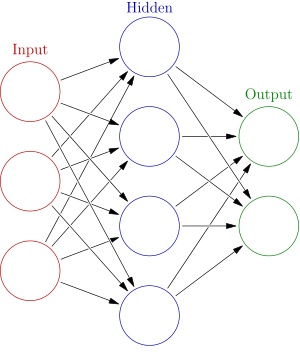
\includegraphics[scale=0.5]{ffnn.png}
    \caption{Feed-forward Neural Network Structure (\textit{From Wikipedia})}
    \label{fig:fnn-struct}
\end{figure}

Then, we will use RNN (recurrent neural network) and LSTM (long-short term memory) architectures to explore the time-dependency between frames. RNN, with neurons taking states from previous time frame(s) as input in addition to the regular input at the current time frame, is especially good at learning from features with sequential properties and does not require fixed input size. LSTM is a derived architecture from RNN. The absence of activation function in its recurrent neurons enables it to capture both long-term and short-term historical features. The structure of RNN and LSTM models are shown in fig. \ref{fig:rnn-struct} and fig. \ref{fig:lstm-struct}, respectively. 

\begin{figure}[h!]
	\centering
    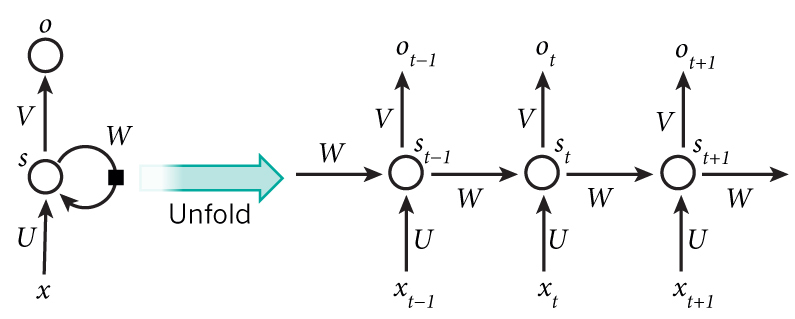
\includegraphics[scale=0.3]{rnn-struct.jpg}
    \caption{Recurrent Neural Network Structure (\textit{From WildML})}
    \label{fig:rnn-struct}
\end{figure}

\begin{figure}[h!]
	\centering
    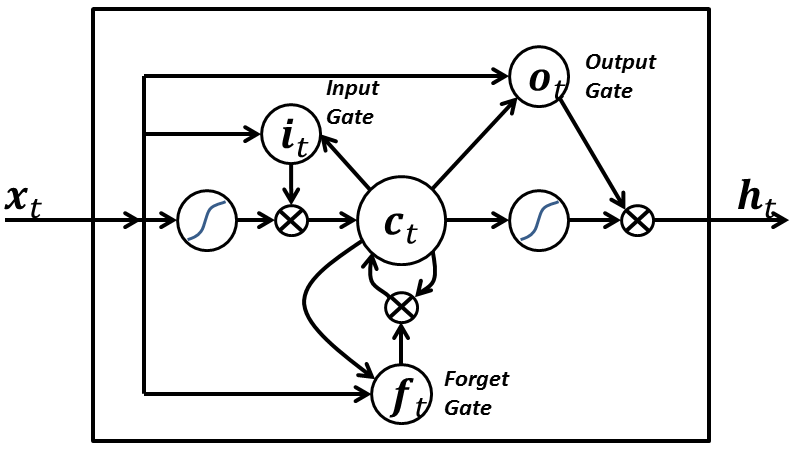
\includegraphics[scale=0.3]{lstm-struct.png}
    \caption{Long-Short Term Memory Neuron Structure (\textit{From Wikipedia})}
    \label{fig:lstm-struct}
\end{figure}

In Mocap classification, since movements are likely to be related to time sequence, and different classes of movement are not necessarily linearly separable with respect to their features from sensors, we consider adopting these time-dependent neural network architecture. \\

% ============================================================================ %
\section{Experiments}

In the experiments, we use eight categories of Mocap data from the CMU Graphics Lab Motion Capture Database. And we will classify from 8 categories: walking, running, jumping, climbing, kicking, swing, boxing, and eating. We choose such a subset with half of the motion involving periodicity and the other half does not. We utilize the data by interpreting the data 62 sensors data as the skeleton movement. We will try to discover the correlation between sensors in each frame using clustering, and relation to time using Recurrent Neural Network. 

% ---------------------------------------------------------------------------- %
\subsection{Time-independent Classification}

We start the experiment on Human Motion Data Classification by exploring the information encoded in a single frame, where contains 62 values from sensors. This can be easily formulated as a multi-class classification problem with 8 categories. We first try to train a Multi-class Support Vector Machine, and then try to train a shallow feed-forward neural network. Finally, we will propose an insight on Human Motion Data. 

\begin{enumerate}
\item \textit{ECOC Multi-class SVM}

For the experiment, we utilized a multi-class Support Vector Machine with Error-correcting Output Model. We randomly select 4000 examples from all the frames of each categories and train the SVM. We were able to obtain an accuracy of 99.1\% in the testing. \\

\item \textit{Feed-forward Neural Network}

The simple three-layer Neural Network we train to classify Human Motion has 64 input neurons with ReLU activation, 32 hidden neurons with ReLU activation, and 8 output neurons corresponding to the categories with Softmax activation. Each input neuron takes vector of dimension $62*window$, where $window$ is a parameter controlling the number frames are concatenated. \\

We change the $window$ and observe how the testing accuracy changes, and we obtain the following graph: 

\begin{figure}[h!]
    \centering
    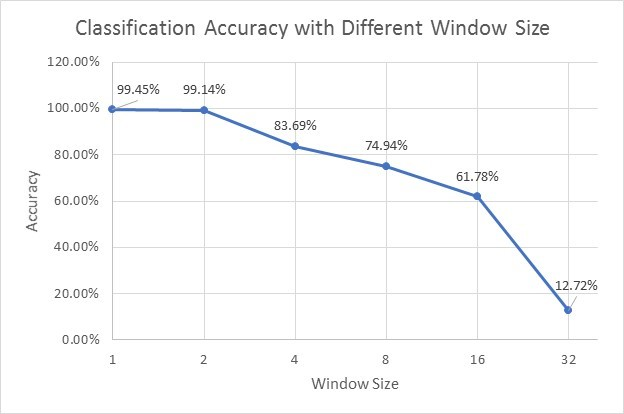
\includegraphics[scale=0.5]{nnac.jpg}
    \caption{Accuracy with Respect to Different Window Size}
\end{figure}

The trend is obvious that as multiple frames are concatenated together, the performance of the 3-layer Neural Network drops. However, as with SVM, the model performs well for a single frame of 62-dim feature vector, achieving $99\%$ accuracy. \\

\item \textit{Clustering}

In this experiment, we use K-Means algorithm to classify randomly chosen 4000 frames 20 times, and calculated the averages. We than analyze the data by examining the structure of the clusters. 

From fig. \ref{fig:cluster1}, we observed that there exists a major type of motion in most clusters. If we examine pairs of clusters or combined clusters, we can typically separate out two motions. From fig. \ref{fig:cluster2}, we found that each motion is scatter into multiple clusters, but as the conclusion above, most of the clusters contain a major type of motion, and inspecting pairs of combined clusters, we could mostly separate two motions. 

\begin{figure}[h!]
    \centering
    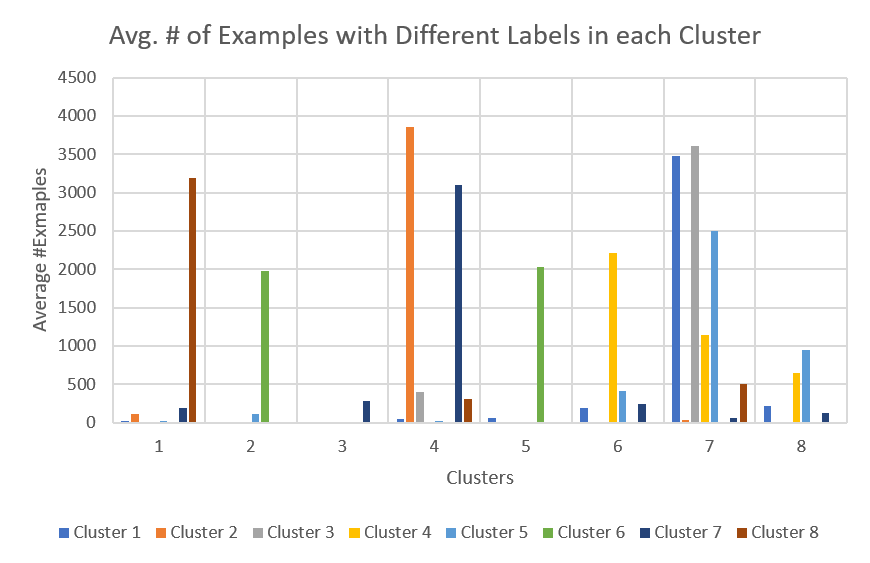
\includegraphics[scale=0.4]{cluster1.png}
    \caption{Average Number of Examples in each Cluster}
    \label{fig:cluster1}
\end{figure}
\begin{figure}[h!]
    \centering
    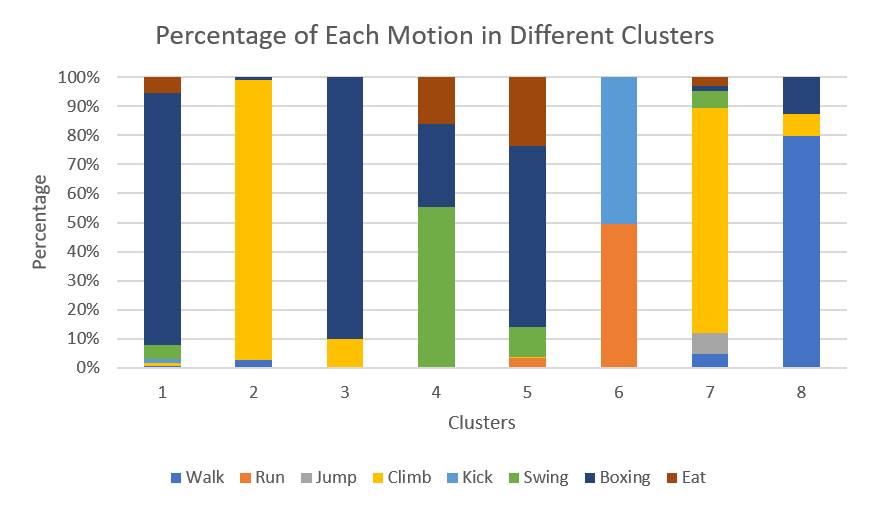
\includegraphics[scale=0.4]{cluster2.png}
    \caption{Percentage of Each Motion Data in Different Clusters}
    \label{fig:cluster2}
\end{figure}

\end{enumerate}

% ---------------------------------------------------------------------------- %
\subsection{Time-dependent Classification}

In the second part of experiment, we use models and algorithms that exploit the time-dependency between contiguous frames. In our RNN model, the first layer consists of 64 recurrent neurons, the second and third layers consist of ReLU-activated perceptrons (64 in the second layer and 32 in the third layer), and the output layer consists of 8 (corresponding to the number of classes) softmax-activated perceptrons. The LSTM model differs from the RNN model in that the first layer is replaced by LSTM neurons. 

After parameter tuning we use $\emph{stride}=16$, $\emph{window}=256$ for both RNN and LSTM. 

Table \ref{tab:nn-acc} shows the accuracy of RNN and LSTM, and fig. \ref{fig:nn-curve} shows the learning curve of the three neural network based algorithms. 

\begin{center}
    \begin{tabular}{|c|c|c|}
        \hline
        Algorithm & Accuracy \\
        \hline
        RNN & 96.25\% \\
        \hline
        LSTM & 99.32\% \\
        \hline
    \end{tabular}
    \captionof{table}{Accuracy of Time-dependent Classification}
    \label{tab:nn-acc}
\end{center}

\begin{figure}[h!]
	\centering
 	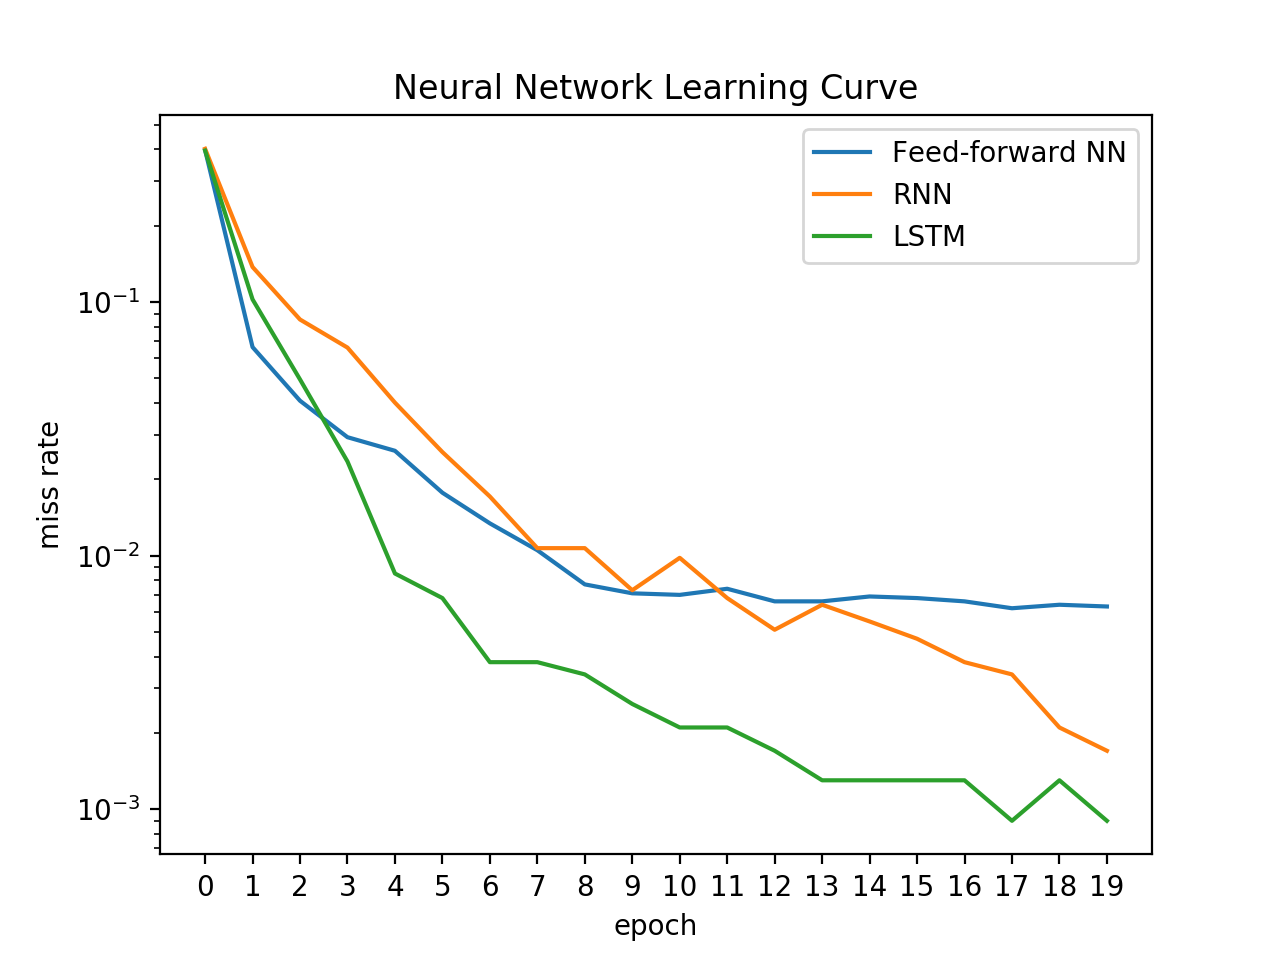
\includegraphics[scale=0.6]{nn_acc.png}
	\caption{Average Number of Examples in each Cluster}
    \label{fig:nn-curve}
\end{figure}

% ============================================================================ %
\section{Discussion}

Intuitively, one cannot classify a motion from just a single frame, we were not expecting $99\%$ accuracy from the time-independent classification. However, we obtained such high accuracy from both SVM and NN models. Therefore, we hypothesized that there must be enough information encoded in each frame; in other words, there must be correlations between 62 sensors that is utilized during training. 

We confirmed the hypothesis by clustering, finding that most clusters contain a major type of motion, and each motion is separated into multiple clusters. Two pairs of combined clusters are highly possibly to be linear separable, or these exists a non-linear decision boundary that correctly classifies two motions. Therefore, the counterintuitive high accuracy of SVM and NN on a single frame could be explained. 

% ============================================================================ %
\section{Conclusion}

All models in the experiments performed well for the chosen eight categories, and classification can be done in real-time.

With relatively few number of categories to classify, frames from different categories could be separated from each other using information encoded in the correlation between sensors. The information encoded is enough to provide the basis to assign the label as evidenced by the high accuracy of SVM and Feed-forward Neural Network.

LSTM has a stable performance during training and testing for various size of dataset. One advantage of utilizing time-dependency is the ability to re-classify and produce a new label once the change in motion is detected by the network.

We have developed a deeper understanding towards the dataset and a modern neural network structure.


% ============================================================================ %
\begin{thebibliography}{99}

\bibitem{c1} H. Kadu, and C.-C. J. Kuo, “Automatic Human Mocap Data Classification,” \textit{IEEE Transactions on Multimedia}, Vol. 16, No. 8, Dec. 2014.
\bibitem{c2} C. Li, P. Kulkarni, L. Liu, B. Prabhakaran, and L. Khan, “Real-time classification of multivariate motion data using support vector machines (SVM),” in \textit{Proc. 5th Int. Workshop Multimedia Data Mining}, 2004, pp. 1–7.
\bibitem{c3} H. Kadu, M. Kuo, and C.-C. J. Kuo, “Human motion classification and management based on mocap data analysis,” in \textit{Proc. Joint ACM Workshop Human Gesture Behavior Understanding}, Dec. 2011, pp. 73–74.
\bibitem{c4} K. He, X. Zhang, S. Ren, and J. Sun, “Deep Residual Learning for Image Recognition,” \textit{Microsoft Research}, Dec. 2015.

\end{thebibliography}

\end{document}
